\indent

Establishing production quality electron beam for experiments in Hall B is a two step process. The initial tune is done at low current by deflecting the beam down to an intermediate dump with the Hall 
B tagged photon spectrometer dipole magnet \cite{tagger}. For higher beam energies, $E>6.12$ GeV, this is newly established beam dump on the tagger dipole magnet yoke. In this case the appropriate field setting for the tagger dipole relates to the beam energy as \cite{yokedump}:
\begin{eqnarray}
I(A)~=~43.491\times E(GeV)-0.076
\end{eqnarray}

In this first step:
\begin{itemize}
\item the CLAS12 detectors (especially tracking detectors) must be OFF 
\item all halo counters must be ON
\item the "blank" collimator is on the beam
\item the CLAS12 solenoid and torus magnets are energized (or can be be energized while beam tune is in progress)
\end{itemize}

The beam with required profile and trajectory is established by MCC ops using correctors and quadrupoles on 2C line, while monitored by Hall-B shift crew using the wire harps and nanoamp (nA) BPMs \cite{nA_BPM} in the upstream tunnel at 2C21 and 2C24 girders (see  Figure \ref{fig:belements}). There is a Yag viewer, ITV2C24, upstream of the tagger dipole controlled by MCC that can also be used to verify the position of the beam. Hall-B shift personnel should work with MCC operator to establish required quality beam. All harp scans must be properly analyzed and logged into logbook. The beam tune is good when required parameters for the profile (x/y widths) and trajectory (x/y positions on various monitors) are achieved (this parameters will be written on the white board in counting house and/or on the run wiki).  

\begin{figure}[htb!]
\centering
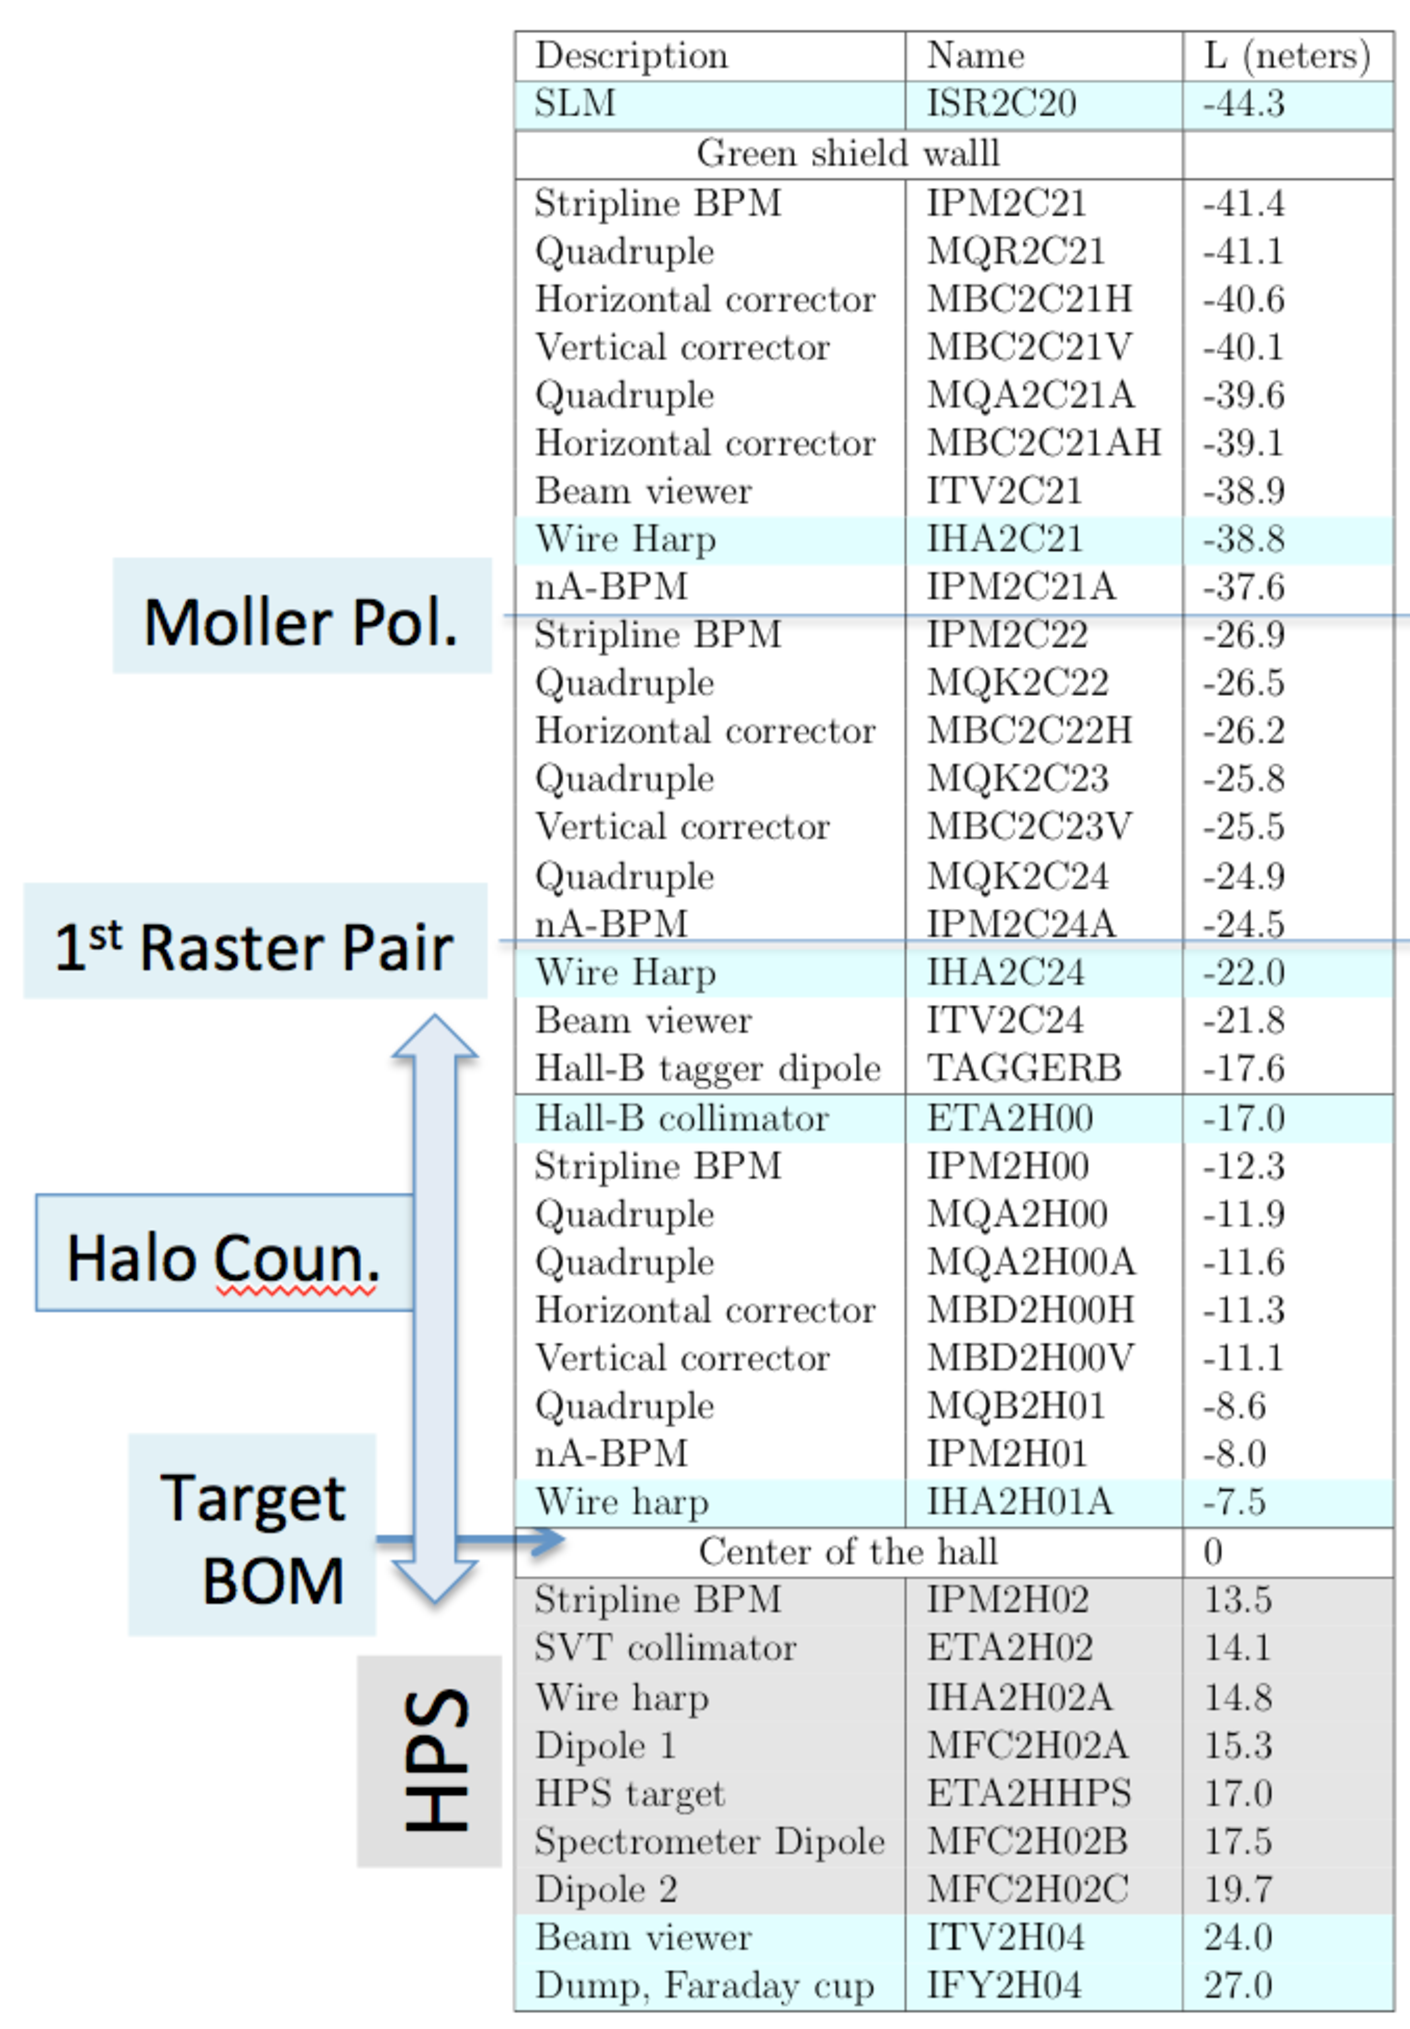
\includegraphics[width=0.8\textwidth]{beamline_elements.pdf}
\caption{Bemaline elements from the green shield wall to Faraday cup dump.}
\label{fig:belements}
\end{figure}

The second step of establishing the physics beam starts after acceptable beam parameters have been achieved on the tagger dump. The following are steps for sending beam to CLAS12:
\begin{itemize}
\item tell MCC that beam is acceptable 
\item ask to degauss and turn OFF the tagged photon spectrometer dipole 
\item position $20$ mm diameter collimator on the beam 
\item when ready ask MCC to send $\sim 5$ nA beam straight to the electron dump at the end of the Hall B beamline, where Faraday cut is located 
\item verify that beam goes to the dump 
\begin{description}
\item[a.] make sure beam is clearly visible on the downstream viewer (use Chromox screen)
\item[b.] make sure that Faraday cup beam current reading and beam current from 2C21 and 2C24 BPMs are consistent (should not be different more then few \%)
\end{description}
\end{itemize}

The beam profile and position adjustments on the target will be done using correctors and quadrupoles on 2C22/2C23/2C24 girders in the upstream tunnel and 2H00 girder in the hall. The last one is the closest to the target ($\sim 10$m upstream) and will be used to focus beam at the target location to achieve required size (preferably $<200~\mu$m). The profile and position of the beam on the CLAS12 target will be checked using the 3-wire harp 2H01A mounted about $5$ meters upstream of the CLAS12 target and 2H01 nA BPM. {\bf During the initial phase of the commissioning, so called KPP run, when $^{12}$C wire target is used, the 2H01A harp will be mounted at the location of the CLAS12 target (carbon wire is actually mounted on the harp stick)}. This harp measures the beam profile and its projected position along x-, y-, and $45^\circ$ axes. After physics quality beam is established, beam position on the cryo target cell must be adjusted based on the lowest rates on the downstream halo counters and BOM. 

After high quality beam was established and properly aligned, 
the beam orbit lock system should be engaged. This system uses position readings from the two stripline BPMs to regulate 
currents in the horizontal and vertical corrector dipoles to minimize beam motion at the target.  The final step in establishing the production running conditions is setting 
limits on the halo counter and BOM rates for the beam Fast Shut Down (FSD) system. If the beam moves close to obstacles, e.g. 
collimator walls or to the thick parts f the target cell windows, count rates on the beam halo monitors and BOM will increase. The appropriate rate limits will depend on actual run conditions and the target, and will be noted on the white board in the counting room and/or on the run wiki.
